\section{Preliminary}
\label{sec:preliminary}

\subsection{Background}
\label{sec:background}

\noindent
\textbf{LLM Agents and the Trust Boundary.} Autonomous language model
agents transition LLMs from passive text generators into goal-driven
systems that iteratively perceive environments, formulate multi-step
plans, and execute programmatic
actions~\cite{react,agentbench,swebench}. Such systems coordinate
three foundational components: a reasoning and planning module that
decomposes user goals into intermediate execution
trajectories~\cite{react}, a tool actuation interface that maps
textual intents into structured API invocations and standardizes
cross-server execution protocols via the Model Context Protocol
(MCP)~\cite{toolformer,mcp,autogen}, and a memory module that
maintains execution state and retrieves historical contexts across
sessions~\cite{memgpt}. This operational loop fundamentally relocates
the system security boundary. While conventional language model
interactions remain restricted to authenticated user prompts, an
autonomous agent continuously populates its context window with
unauthenticated external observations, including web retrieval
results, repository files, API payloads, and third-party MCP tool
outputs~\cite{mcpsafetyaudit,mcpfirstglance}. Consequently, external
data streams become directly entangled with the internal instruction
flow of the agent, exposing the execution environment to
unauthenticated third-party content during standard operation.

\noindent
\textbf{Injection and Jailbreaking Attacks on LLM Agents.}
Autoregressive transformers typically lack a built-in mechanism to separate
control instructions from data payloads, as they process all inputs
homogeneously as a continuous token
sequence~\cite{perez-ribeiro,greshake}.
Adversaries exploit this
limitation via prompt injection, where malicious instructions in user
inputs (direct injection) or external resources such as web pages,
files, and API responses (indirect injection) hijack the agent
execution trajectory~\cite{perez-ribeiro,greshake,injecagent,
tensortrust}. In parallel, jailbreak attacks bypass safety alignment
through persona adoption, linguistic obfuscation, or adversarial token
optimization, composing with indirect injections to force the
invocation of privileged tools~\cite{wei-jailbroken,zou-gcg,shen-dan}.
Beyond runtime prompt manipulation, adversaries employ data and state
poisoning to induce persistent compromise across the agent lifecycle.
This includes corrupting instruction-tuning
datasets~\cite{wan-poisoning}, poisoning retrieval-augmented
generation knowledge bases~\cite{poisonedrag,ragroll}, backdooring
episodic memory stores~\cite{agentpoison,asb}, and returning malicious
MCP tool responses that steer agents toward unauthorized code
execution and credential
theft~\cite{mcpsafetyaudit,mcpfirstglance,toolsword}. Incidents such as
EchoLeak (\texttt{CVE-2025-32711}) against Microsoft 365
Copilot~\cite{cve202532711,echoleak} and command injection
vulnerabilities in GitHub Copilot (\texttt{CVE-2025-53773},
\texttt{CVE-2026-29783})~\cite{cve202553773,cve202629783} demonstrate
the severity of these attack vectors.


\noindent
\textbf{Defensive Methodologies.} Existing defensive literature
addresses agent manipulation across three primary paradigms: input
filtering, model hardening, and system-level isolation. Input-level
defenses inspect candidate text before admission into the context of
the agent, utilizing regular expressions and programmable
guardrails~\cite{nemoguardrails}, compact sequence classifiers such as
Llama Prompt Guard, Protect AI DeBERTa, and Llama
Guard~\cite{promptguard,protectaideberta,llamaguard}, auxiliary
LLM-as-a-judge evaluators~\cite{zheng-judge}, canary-based
known-answer verification~\cite{liu-injection}, or game-theoretic
minimax detectors such as
DataSentinel~\cite{datasentinel}. Model-level defenses harden internal
representations against adversarial instructions through syntactic
transformations such as Spotlighting~\cite{spotlighting}, hierarchical
instruction tuning that prioritizes developer directives over
untrusted observations~\cite{instructionhierarchy}, structured query
delimiters via StruQ~\cite{struq}, and preference optimization via
SecAlign~\cite{secalign}. System-level defenses enforce execution
constraints at runtime, including spoke-based application
compartmentalization in IsolateGPT~\cite{isolategpt}, capability-based
information flow tracking in CaMeL~\cite{camel}, and structural policy
enforcement on tool invocations in AgentWard and
ClawGuard~\cite{agentward,clawguard}. However, existing defenses face
persistent trade-offs among runtime efficiency, detection precision,
and post-deployment adaptability, as static rules remain brittle
against semantic evasion while heavyweight evaluators and manual
policies cannot dynamically absorb novel attack variations.


\subsection{Threat Model}
\label{sec:threat-model}

\noindent
\textbf{System and Trust.} We consider a tool-augmented
LLM agent that performs open-ended tasks on behalf of a benign user.
The agent plans actions, invokes local and remote tools, and consumes
external observations through untrusted channels, including web search
results, local files, API responses, and MCP tool
outputs~\cite{agentdojo,injecagent,mcpsafetyaudit,mcpfirstglance}. The user prompt is trusted:
the user is not adversarial and does not intentionally provide
malicious instructions. External content referenced by the prompt
remains untrusted. The trusted computing base (TCB) comprises the agent
host runtime, the underlying model or model service, and the
CAITLYN daemon together with its defense
repository\footnote{An analysis of security risks regarding the
defense repository of CAITLYN itself is provided in
Appendix~\ref{app:repository-risks},
and discussions on the derived adaptive attacks are presented in
Section~\ref{sec:AdaptiveAttacks}.}. Untrusted channels are mediated
by CAITLYN: modern LLM agents natively support event hooks or
middleware interfaces, so external inputs entering the agent context
trigger a CAITLYN inspection unless there are any engineering
implementation issues (i.e., hook time out).
This aligns with the standard trust model of AgentDojo, InjecAgent, and
CaMeL~\cite{agentdojo,injecagent,camel}.

\begin{figure*}[!ht]
  \centering
  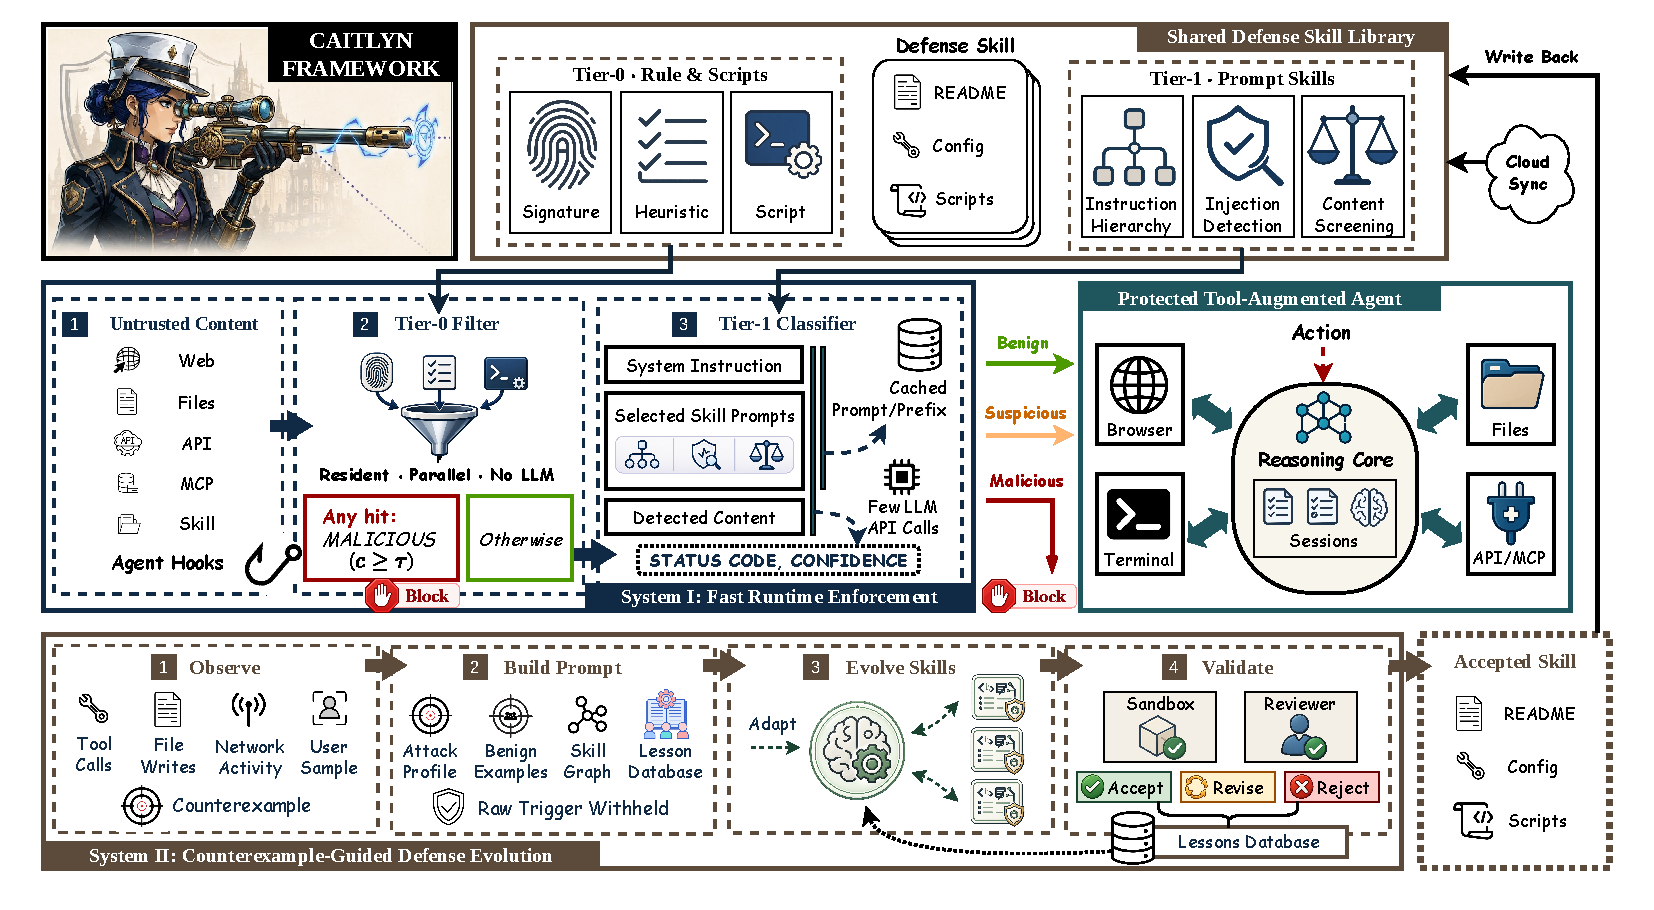
\includegraphics[page=1,width=\textwidth]{figs/method.drawio.pdf}
  \caption{
    The overall framework of CAITLYN. System~I performs fast
    runtime enforcement with the Tier-0 filter and the Tier-1 classifier
    over untrusted content entering the protected tool-augmented agent,
    while System~II continuously evolves defense skills from observed
    counterexamples and writes them back into the shared defense skill
    library.
  }
  \label{fig:method-framework}
\end{figure*}


\noindent
\textbf{Adversary Objective.} An external adversary seeks to induce
control-flow or data-flow violations in the execution of the agent,
classified into two primary security impacts: confidentiality
violations (exfiltrating private user data, memories, or files to
adversary-controlled endpoints) and integrity violations (triggering
unauthorized state modifications, arbitrary command execution, or
privileged tool invocations with malicious
arguments)~\cite{mcpsafetyaudit,cve202532711,echoleak,cve202553773,cve202629783}.
Conversely, passive task failure or benign output
degradation without unauthorized tool execution falls outside the
security objective~\cite{agentdojo,camel}. When an agent has no
reliable tool channel, the evaluation delivers the payload as
environment content embedded in the prompt; that prompt segment is
treated as an untrusted observation and is monitored by the defense,
consistent with the trusted primary user prompt assumption.

\noindent
\textbf{Adversary Capabilities.} The adversary can write arbitrary
text into untrusted data sources accessed by the agent, including web
pages, repository contents, shared files, API endpoints, and
third-party MCP server
responses~\cite{greshake,liu-injection,tensortrust}. Payloads may
incorporate linguistic obfuscation, semantic indirection, multi-stage
framing, or jailbreak patterns to evade detection. We assume a strong
adversary who possesses black-box query access and knowledge of the
tool interfaces and parameter schemas of the agent, enabling targeted
payload crafting~\cite{agentdojo,injecagent}. The adversary can observe
public outputs and tool execution traces to refine evasion strategies
over time. The adversary cannot modify the system prompt
of the agent and cannot alter the weights or API credentials of the model.

\noindent
\textbf{``Emerging'' Attacks.} An attack vector is defined as \emph{emerging} if
its structural patterns, evasion mechanisms, and payload distributions
are disjoint from the initial defense repository at deployment
time. Specifically, an emerging attack is absent from the curated seed
attack corpus, was not used during the authoring or verification of
baseline defense skills, and is not matched by the seeded heuristic
signatures. The open-world operational environment allows adversaries
to introduce novel attack families continuously after
deployment. Under this formulation, the threat model evaluates whether
a minimal number of observed counterexample encounters (e.g., logged
bypasses or incident reports) provides sufficient specification for
the defense to autonomously synthesize verified, effective
countermeasures without compromising benign task utility.
While formal guarantees of completeness against unconstrained future
payloads remain beyond the reach of empirical synthesis, concrete
mitigation rates across emerging attack families are empirically
evaluated in Section~\ref{sec:EmergingBenchmark}.
